Pour pouvoir déclarer un centre de vacances, développez le secteur \ovalbox{centre de vacances} depuis le volet de navigation, puis cliquez sur l'entrée \ovalbox{Activités}. Cela vous mènera vers la liste de vos activités\footnote{Par défaut, le Portail Pro affiche les activités de l'année budgétaire ONE (l'année budgétaire commence avec les vacances d'hiver et se termine avec le congé d'Automne). Vous pouvez changer l'année budgétaire en haut à droite.}. Cliquez ensuite sur \ovalbox{Nouvelle activité}. 

Vous pouvez également utiliser le raccourci depuis la page d'accueil. Cependant le raccourci vous mène directement vers le formulaire, nous vous conseillons plutôt de d'abord consulter vos activités centres de vacances afin éviter d'encoder un doublon de déclaration.  


\centerline{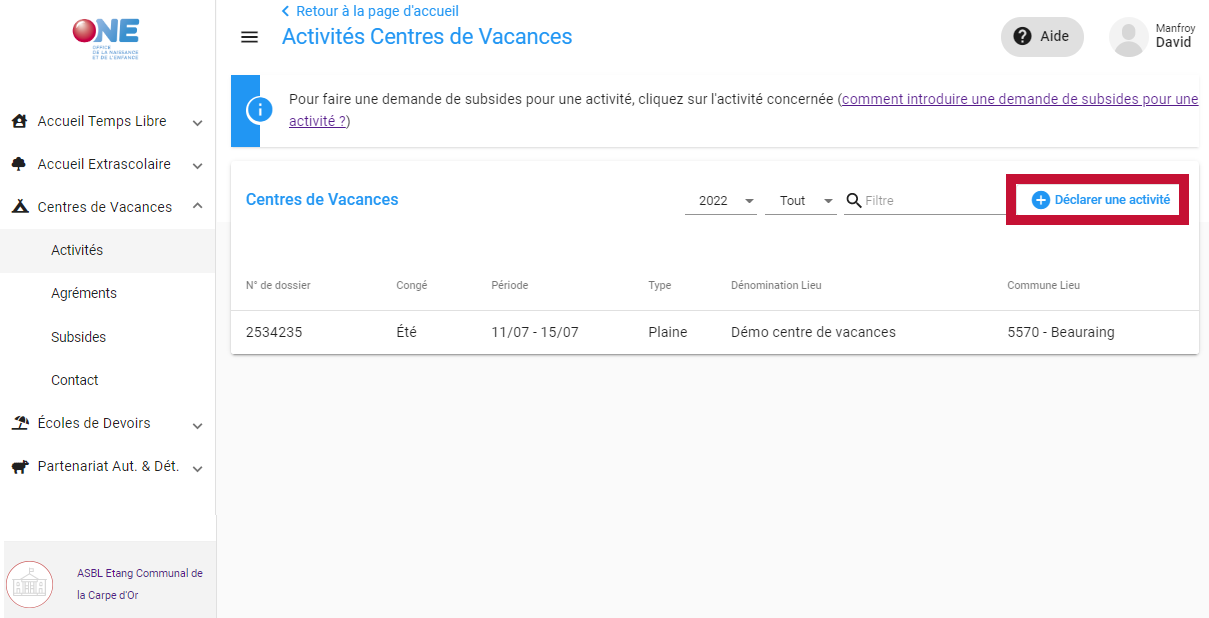
\includegraphics[width=14cm]{Images/cdv/liste_acti_cdv.png}}


\subsection{DA - Renseigner les caractéristiques de l'activité}
\begin{itemize}
    \item Choisissez \textbf{l'agrément correspondant} (plaine ou séjour), le type d'activité en sera déduit automatiquement.
    \item Cochez le(s) \textbf{type(s) d'accueil applicable} (âge des enfants, avec handicap, spécialisé) et renseignez le tarif standard pour  \textbf{la participation aux frais demandée aux parents}\footnote{Si vous avez plusieurs tarifs, renseignez ici le tarif le plus haut appliqué. L'éventuel détails des modes de tarification doit être spécifié dans le règlement d'ordre intérieur (ROI)}.
    \item Ajoutez les \textbf{périodes de l'activité}: si possible ajoutez les plages de dates précises de vos activités (en excluant les congés ou les jours de fermeture). Pour les plaines de vacances, \textbf{ajoutez les heures d'ouverture}.
\end{itemize} 

\begin{figure}[ht]
    \centering
    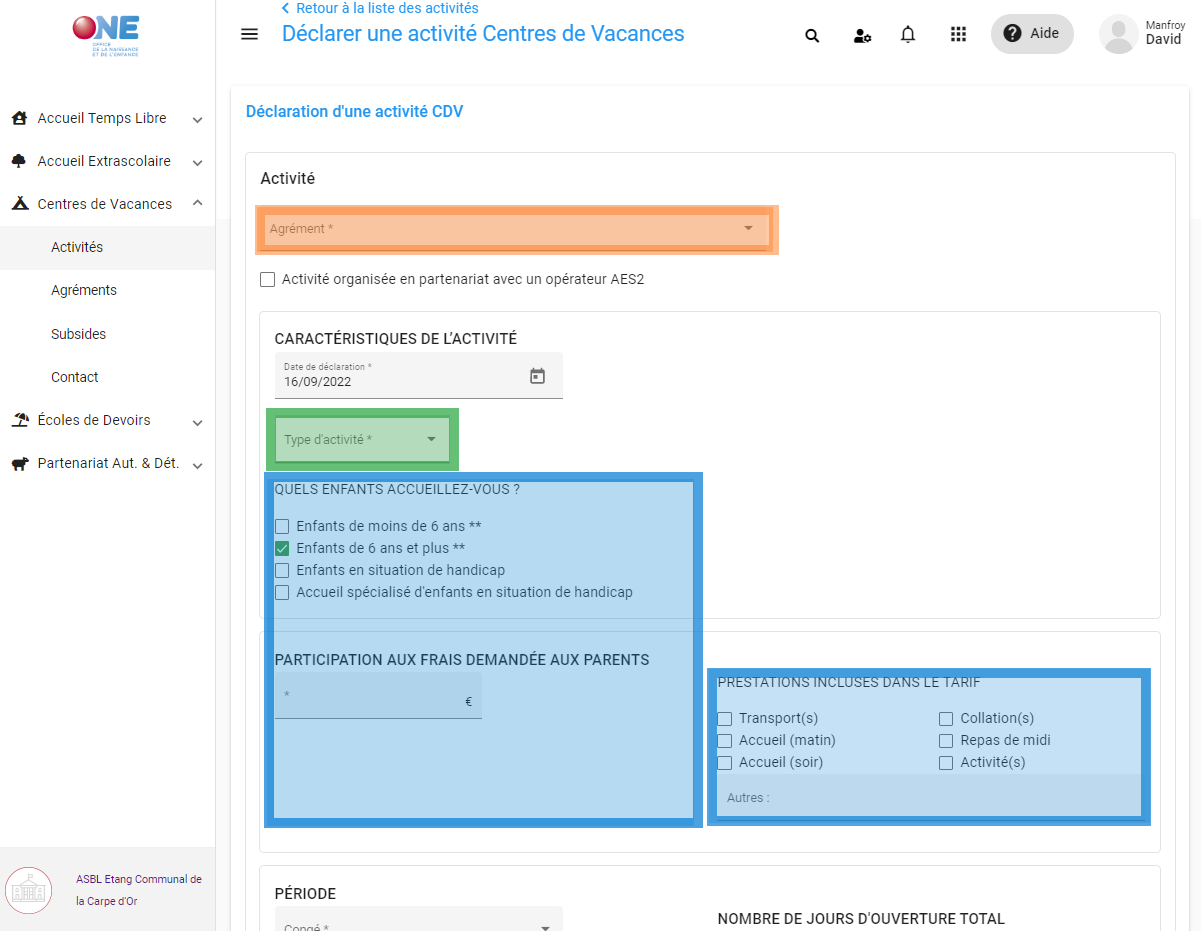
\includegraphics[width=12cm]{Images/cdv/da-acti.png}
    \caption{Formulaire de déclaration d'activités: caractéristique d'accueil de votre centre de vacances}
    \label{fig:cdv_da}
\end{figure}


\subsection{DA - Renseigner les informations sur le lieu}
\begin{itemize}
    \item Ajoutez la \textbf{dénomination} et l'\textbf{adresse} de votre centre de vacances.
    \item Enregistrez un ou plusieurs \textbf{coordinateur(s) du centre}. Si vous n'avez pas encore défini de coordinateur à la date de votre déclaration, vous pouvez passer à l'étape suivante. N'oubliez pas de le renseigner ultérieurement à votre gestionnaire de dossier avant le début du centre. 
\end{itemize}


\begin{figure}[h]
    \centering
    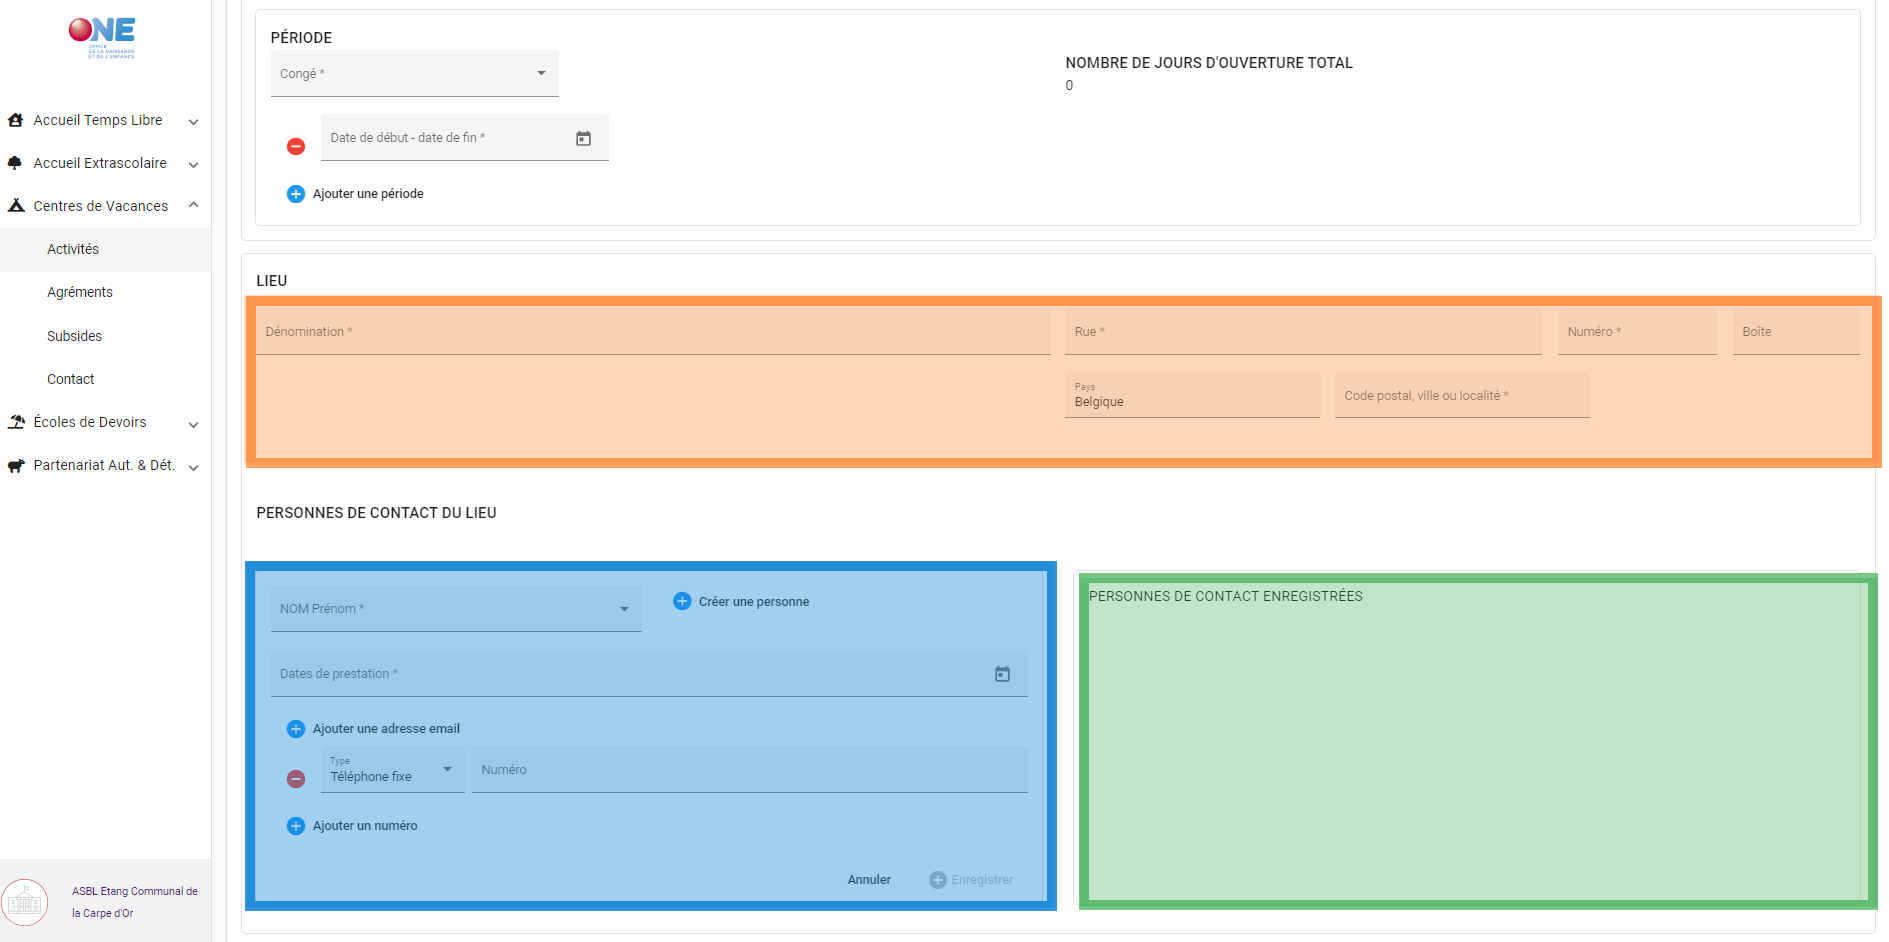
\includegraphics[width=12cm]{Images/cdv/da-lieu.png}
    \caption{Formulaire de déclaration d'activité: description du centre de vacances et coordonnées de la personne de contact ou du coordinateur du centre physiquement sur place.}
    \label{fig:cdv_da2}
\end{figure}


Si vous devez mettre à jour une information de votre déclaration (apporter une correction ou renseigner votre nouveau coordinateur par exemple), contactez votre gestionnaire de dossier. A ce stade, seuls nos agents peuvent modifier les informations de la déclaration d'activité. 
\section{Détails d'une activité centre de vacances déclarée}

Vos déclarations d'activité sont enregistrées dans la liste de vos activités centres de vacances. 

Depuis la liste de vos activités, si vous cliquez sur la ligne d'un de vos centres déclarés, vous ouvrirez le détail de l'activité.

\textbf{Plusieurs onglets sont disponibles:} 

\centerline{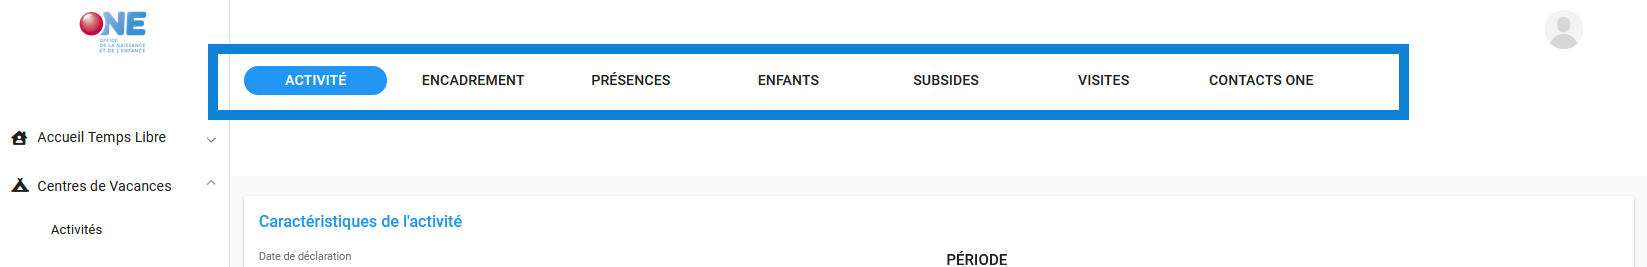
\includegraphics[width=13cm]{Images/cdv/cdv-onglets.png}}

\begin{itemize}[label=\textbullet,font=\color{bleu}]
    \item \ovalbox{\textbf{Activité}}: le résumé de votre déclaration. Pour mettre à jour les informations, prenez contact avec votre gestionnaire de dossier. 
    \item \ovalbox{\textbf{Encadrements}}: le personnel d'encadrement de votre centre de vacances;
    \item \ovalbox{\textbf{Présences}}: les présences des encadrants et des enfants;
    \item \ovalbox{\textbf{Enfants}}: liste des enfants et nombre d'enfants accueillis; 
    \item \ovalbox{\textbf{Subsides}}: pour envoyer votre demande de subsides (après avoir complété les onglets encadrement, présences et enfants, voir le point \ref{DS_CDV});
    \item \ovalbox{\textbf{Visites}}: pour consulter les rapports de visites (coordinateur accueil de l'ONE);
    \item \ovalbox{\textbf{Contact}}: les coordonnées de votre gestionnaire de dossier, de votre inspecteur comptable et de votre coordinateur accueil. 
\end{itemize}